\chapter{Genome assembly of Candida nivariensis}
\label{chap:nivar}

\textbf{Portions of this chapter originally appeared in:} \\
Fan Y, Gale AN, Bailey A, Barnes K, Colotti K, Mass M, et al. Genome and transcriptome of a pathogenic yeast, Candida nivariensis. G3 Genes|Genomes|Genetics. 2021;11. doi:10.1093/g3journal/jkab137

\section{Abstract}
\label{sec:abstract}

We present a highly contiguous genome and transcriptome of the pathogenic yeast, Candida nivariensis. We sequenced both the DNA and RNA of this species using both the Oxford Nanopore Technologies and Illumina platforms. We assembled the genome into an 11.8 Mb draft composed of 16 contigs with an N50 of 886 Kb, including a circular mitochondrial sequence of 28 Kb. Using direct RNA nanopore sequencing and Illumina cDNA sequencing, we constructed an annotation of our new assembly, supplemented by lifting over genes from Saccharomyces cerevisiae and Candida glabrata.

\section{Introduction}
\label{sec:intro}

For immunocompromised hosts, opportunistic infections caused by drug-resistant fungi of the Candida genus are a major source of morbidity and mortality \citep{Borman2008-cr}. In particular, Candida nivariensis, a close relative to Candida glabrata, has emerged in recent years as especially resistant to antifungal therapies \citep{Borman2008-cr}. However, due to its phenotypic similarities to C. glabrata, C. nivariensis is generally underidentified and easily misdiagnosed, and currently, only molecular approaches can distinguish the two \citep{Aznar-Marin2016-yp}, spurring whole-genome sequencing studies on the clade \citep{Gabaldon2013-bk}.

Accurate assembly of repetitive genomic regions is crucial for understanding genetic diversity and virulence in pathogenic species. Fungal pathogens have long been known to exhibit a high degree of genome plasticity to enhance fitness in various environments \citep{Croll2013-mm, Ford2015-qs, Lopez-Fuentes2018-zt, Carrete2019-xo, Todd2019-sy}. Repetitive subtelomeric regions in particular play a crucial role in virulence for many pathogenic organisms \citep{Barry2003-ln, De_Las_Penas2003-zd}. Many yeasts’ subtelomeric regions contain and regulate the expression of genes crucial for biofilm formation, carbohydrate utilization, and cellular adhesion \citep{Naumov1995-ju,  De_Las_Penas2003-zd, Iraqui2005-hy}. These gene families often undergo rapid evolution through changes in copy number and sequence through either SNPs or indels \citep{Carreto2008-pz, Brown2010-az, Anderson2015-fa}. However, these subtelomeric regions remain one of the most difficult sections of the genome to accurately assemble due to their repetitive nature and high sequence similarity between genes, making genetic analysis cumbersome \citep{Brown2010-az}.

One of the gene families of great interest to the pathogenic yeast field are the GPI-anchored cell wall proteins. This protein family includes many genes that encode for adhesion proteins that are found in various members of the Candida genus, and play a key role in pathogenicity, being involved in regulation of biofilm formation, cell-to-cell contact, and host-pathogen interactions \citep{Timmermans2018-ci, McCall2019-zn}. With the many roles these genes play in infection, the accurate identification and understanding of the genetic variation of these genes vital to combating fungal pathogens.

Unfortunately, like many eukaryotic pathogens, the current reference genome for C. nivariensis (GenBank: GCA\_001046915.1) is highly fragmented. Constructed from sequencing of strain CBS9983, the reference genome consists of 123 contigs with an N50 of 248Kb \citep{Gabaldon2013-bk}, meaning that at least half of the total genome length is contained in contigs 248Kb or longer. This is typical of genomes assembled from limited short-read sequencing data; though short reads are highly accurate, assembling them into contiguous genomes is challenging depending on the size and complexity of the genome. Such short read assemblies have limited utility since large scale variants, repetitive regions, and genome structure remain difficult to elucidate, though they are often involved in the genome plasticity of pathogenic yeasts \citep{Carrete2018-xm}. In contrast, long-read sequencing data has been shown to produce much more contiguous assemblies, and have been crucial in sequencing through large repetitive regions, as well as assessing structural variants. However, read accuracy on the ONT platform in particular ranges from 86% for early basecaller versions \citep{Wick2019-pa} to 97% as currently reported by ONT.  This is lower than the read accuracy of short-read Illumina sequencing, which achieves 99.9% accuracy \citep{Fox2014-li}.  In consensus sequences, most random errors can be corrected by other reads covering the same genomic loci, resulting in >99% consensus accuracy \citep{Wick2019-pa}. However, systematic errors occurring in most or all of the reads cannot be corrected this way. For ONT data, indels at homopolymers dominate systematic errors \citep{Wick2019-pa}. These persistent errors can be problematic for gene prediction and annotation in downstream analysis \citep{Watson2019-tk} and are typically corrected with more accurate short-read data in mappable regions \citep{Garrison2012-iq, Walker2014-eh, Vaser2017-zk}.

Having a genome alone is not enough; we need to annotate it with genes and other functional elements for the genome to be of greatest use. Knowledge of gene loci is critical to constructing phylogenetic relationships between organisms, and to studying the functional implications of variants, both common uses of reference genomes. While model-based, purely computational gene predictors can be highly accurate in bacteria, gene sparsity and intronic regions make this task more difficult in eukaryotes \citep{Salzberg2019-hw}. For improved annotations, some RNA-seq information is required \citep{Salzberg2019-hw}.

Here, as part of our newly developed Methods in Nucleic Acid Sequencing university course, we used a hybrid approach, applying long-read nanopore sequencing to assemble a highly contiguous genome of C. nivariensis, followed by short-read sequencing to polish or correct errors in our assembly. We followed this by a combination of nanopore direct RNA sequencing as well as short-read RNA-seq to annotate our assembly. By combining this data with liftover of annotations from evolutionary “cousins” of nivariensis, we have generated a new and annotated reference genome for the community.


\begin{kframe}
\begin{alltt}
\hlstd{what} \hlkwb{<-} \hlstr{"figure"}
\hlstd{figname} \hlkwb{<-} \hlstr{"asms"}
\hlstd{title} \hlkwb{<-} \hlstr{"Characteristics of the JHU_Cniv_v1"}
\hlstd{desc} \hlkwb{<-} \hlstr{"\{\textbackslash{}\textbackslash{}bf (A)\} Cumulative lengths of the 50 longest sequences in our assembly and previous reference genome. \{\textbackslash{}\textbackslash{}bf (B)\} Ideogram of assembly. Sequence that is missing in the reference genome is shown along each nonmitochondrial contig, and the positions of telomere repeats are marked."}
\hlstd{shortname} \hlkwb{<-} \hlstr{"fig:asms"}
\hlstd{where} \hlkwb{<-} \hlstr{"[!ht]"}

\hlstd{figstr} \hlkwb{<-} \hlkwd{paste0}\hlstd{(}\hlstr{'\textbackslash{}\textbackslash{}begin\{'}\hlstd{, what ,}\hlstr{'\}'}\hlstd{, where ,}\hlstr{'
\textbackslash{}\textbackslash{}centering
\textbackslash{}\textbackslash{}includegraphics[width = 1\textbackslash{}\textbackslash{}linewidth,keepaspectratio]\{figure/'}\hlstd{, figname,} \hlstr{'.pdf\}
\textbackslash{}\textbackslash{}caption['}\hlstd{, title ,}\hlstr{']\{\{\textbackslash{}\textbackslash{}bf '}\hlstd{, title  ,}\hlstr{'.\} '}\hlstd{, desc ,}\hlstr{' \}
\textbackslash{}\textbackslash{}label\{'}\hlstd{, shortname ,}\hlstr{'\}
\textbackslash{}\textbackslash{}end\{'}\hlstd{, what ,}\hlstr{'\}
'}\hlstd{)}
\hlkwd{cat}\hlstd{(figstr)}
\end{alltt}
\end{kframe}\begin{figure}[!ht]
\centering
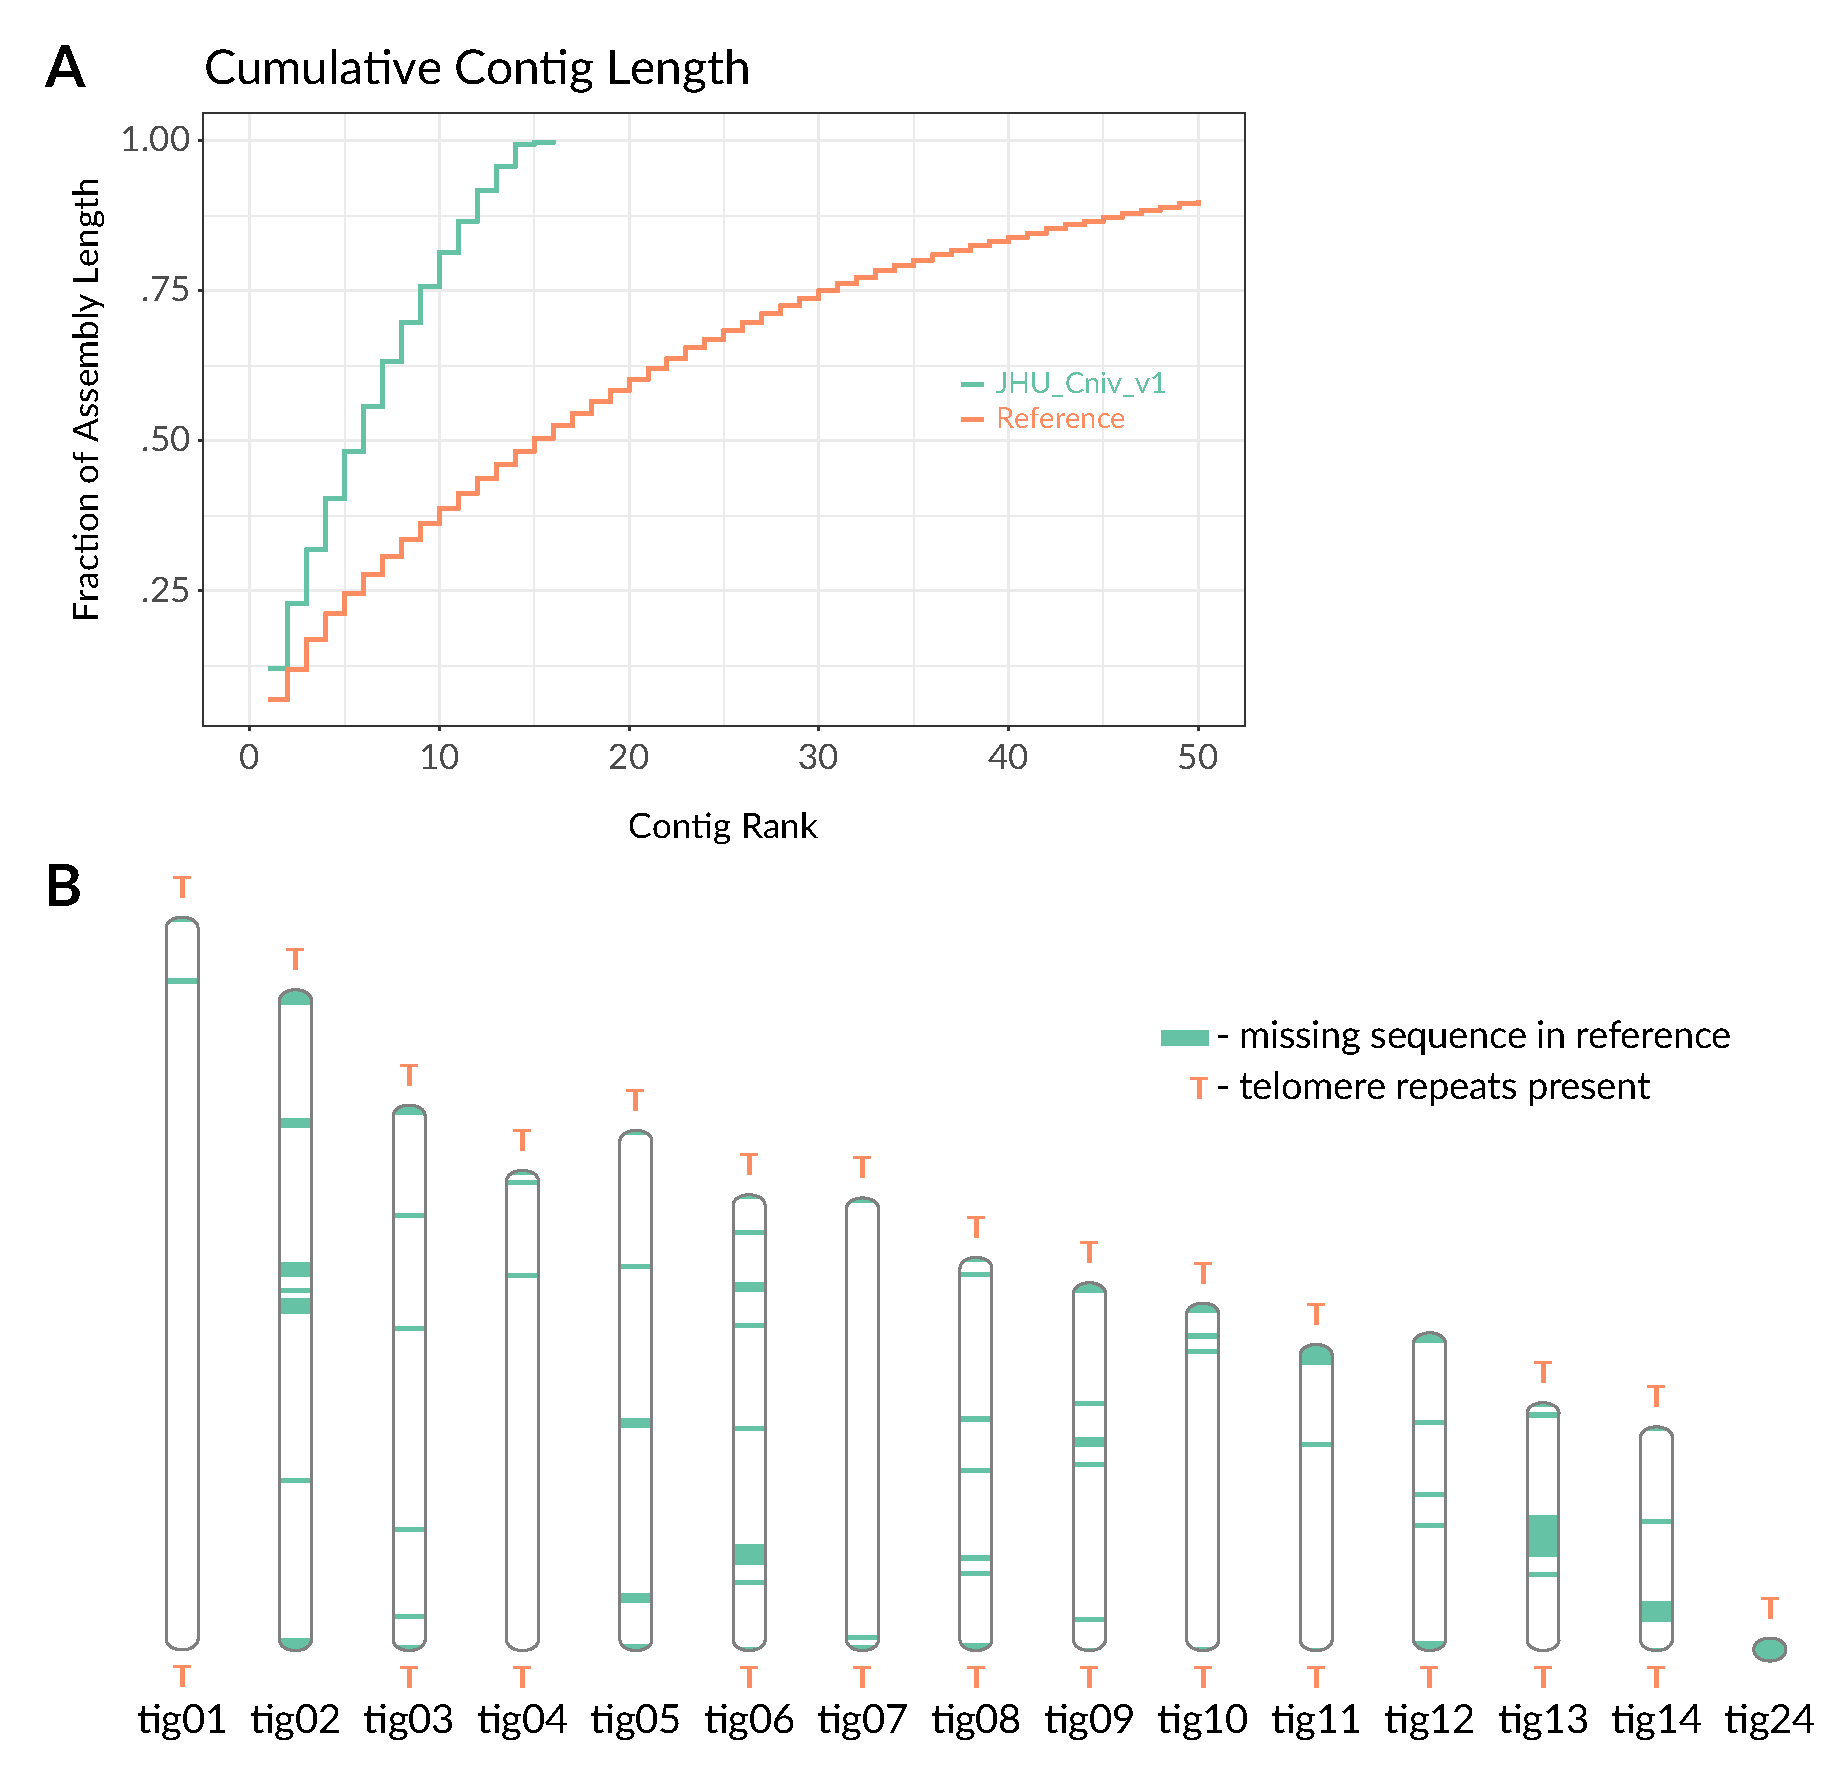
\includegraphics[width = 1\linewidth,keepaspectratio]{figure/asms.pdf}
\caption[Characteristics of the JHU_Cniv_v1]{{\bf Characteristics of the JHU_Cniv_v1.} {\bf (A)} Cumulative lengths of the 50 longest sequences in our assembly and previous reference genome. {\bf (B)} Ideogram of assembly. Sequence that is missing in the reference genome is shown along each nonmitochondrial contig, and the positions of telomere repeats are marked. }
\label{fig:asms}
\end{figure}

